\section{Realisation}
Schon bei Projektstart wurde klar, dass es sich um sehr umfangreiche Anforderungen handelt. Es galt nicht nur eine Streaming Lösung zu implementieren, sondern es mussten auch alle Hardwarekomponenten getestet und angesteuert werden. Für die Bedienerseite musste eine funktionale Webseite einschließlich Webserver erstellt werden und ein Streaming-Server für die Konvertierung und Vernetzung der Sender und Empfänger musste konfiguriert werden. Viele \textbf{wichtige} bisher nicht genannte Anforderungen, z.B. Cybersicherheit, Authentifizierung wurden weitestgehend außer acht gelassen. Sie sind natürlich für eine endgültige industrielle Anwendung unerlässlich.\\

Das Projekt wurde in Teil-Aufgaben realisiert:
\begin{itemize}
\item Inbetriebnahme aller Hardwarekomponenten

\item Direktes Streamen von Audio und Video von embedded System an PC
\item Aufsetzen eines Webservers im lokalen Netzwerk, lokales hosting der Webseite
\item Aufsetzen eines Streaming-Servers im lokalen Netzwerk
\item Direktes Streamen von Audio und Video von embedded System an Streaming-Server
\item Anzeige des konvertierten Outputs des Streaming-Servers auf der Webseite

\item Streamen der PC Webcam an lokalen Streaming-Server
\item Zurück-Streamen vom Streaming-Server an embedded Hardware und Visualisierung

\item Hochladen der Webseite auf eine Online-Webspace
\item Aufsetzen eines Online-Streaming-Servers
\end{itemize}

\subsection{Hardware Inbetriebnahme der Komponenten}
Beschreibung...\\

\subsection{Streamen vom embedded System: Streaming-Server \& Webserver}
Beschreibung...\\

\textbf{Direktes StreamEN von Audio und Video von embedded System an PC}\\
blah blah blah\\

\textbf{Aufsetzen eines Webservers im lokalen Netzwerk, lokales hosting der Webseite}\\
blah blah blah\\

\textbf{Aufsetzen eine Streaming-Servers im lokalen Netzwerk}\\
blah blah blah\\

\textbf{Direktes Streaming von Audio und Video von embedded System an Streaming-Server}\\
blah blah blah\\

\subsection{Webseite zur Anzeige der Videostreams}
Beschreibung...\\

\textbf{Anzeige des konvertierten Outputs des Streaming-Servers auf der Webseite}\\
blah blah blah\\

\subsection{Streamen von PC: Streaming-Server \& Anzeige auf embedded Sytem}
Beschreibung...\\

\textbf{Streamen der PC Webcam an lokalen Streaming-Server}\\
blah blah blah\\

\textbf{Zurück-Streamen vom Streaming-Server an embedded Hardware und Visualisierung}\\
blah blah blah\\

\subsection{Online Setup}
Beschreibung...\\

\textbf{Hochladen der Webseite auf eine Online-Wespace}\\

Hochladen der Webseite via Filezilla...\\

\textbf{Aufsetzen eines Online-Streaming-Servers}\\
blah blah blah\\

\textbf{Webserver Verbindungstest}\\
Im oberen Bereich ist der gstreamer Befehl mit dem Audio udpsink host...5000 und Video udpsink...5001. Wireshark detektiert ankommende Pakete im Webserver (ip 85.214.211.169) vom raspberry pi (ip 77.14.37.230) an den UDP Ports 5000 (Audio Paketgröße 451) und UDP 5001 (Video Paketgröße 894).\\

\begin{minipage}{\textwidth}
    \begin{center}
        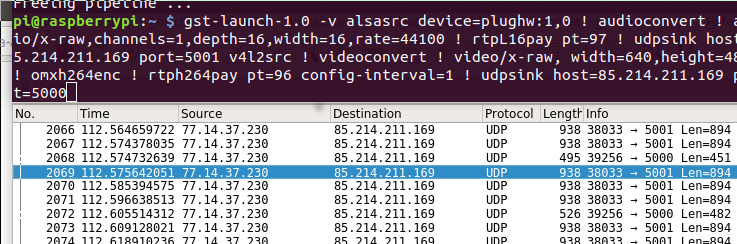
\includegraphics[scale=0.85]{img/wireshark.png} 
    \end{center}
\end{minipage}
